\documentclass[10pt,twocolumn]{article}
% Shared two-column preamble for the three research papers.
% Use with: \documentclass[10pt,twocolumn]{article}
% Then in main.tex: % Shared two-column preamble for the three research papers.
% Use with: \documentclass[10pt,twocolumn]{article}
% Then in main.tex: % Shared two-column preamble for the three research papers.
% Use with: \documentclass[10pt,twocolumn]{article}
% Then in main.tex: \input{../../shared/latex/twocolumn_preamble.tex}

\usepackage[margin=0.75in]{geometry}
\usepackage[utf8]{inputenc}
\usepackage[T1]{fontenc}
\usepackage{lmodern}
\usepackage{microtype}
\usepackage{amsmath,amssymb,amsthm}
\usepackage{graphicx}
\usepackage{booktabs}
\usepackage{caption}
\usepackage{subcaption}
\usepackage{hyperref}
\usepackage{url}
\usepackage{xcolor}
\usepackage{algorithm}
\usepackage{algorithmic}
\usepackage{multirow}
\usepackage{titlesec}
\usepackage{authblk}

\hypersetup{colorlinks=true,linkcolor=blue!50!black,citecolor=blue!50!black,urlcolor=blue!50!black}

\titleformat{\section}{\normalfont\large\bfseries}{\thesection}{0.6em}{}
\titleformat{\subsection}{\normalfont\bfseries}{\thesubsection}{0.5em}{}

\captionsetup{font=small,labelfont=bf,skip=4pt}
\setlength{\columnsep}{0.25in}
\setlength{\parskip}{2pt}

\newtheorem{theorem}{Theorem}
\newtheorem{proposition}[theorem]{Proposition}
\newtheorem{definition}[theorem]{Definition}


\usepackage[margin=0.75in]{geometry}
\usepackage[utf8]{inputenc}
\usepackage[T1]{fontenc}
\usepackage{lmodern}
\usepackage{microtype}
\usepackage{amsmath,amssymb,amsthm}
\usepackage{graphicx}
\usepackage{booktabs}
\usepackage{caption}
\usepackage{subcaption}
\usepackage{hyperref}
\usepackage{url}
\usepackage{xcolor}
\usepackage{algorithm}
\usepackage{algorithmic}
\usepackage{multirow}
\usepackage{titlesec}
\usepackage{authblk}

\hypersetup{colorlinks=true,linkcolor=blue!50!black,citecolor=blue!50!black,urlcolor=blue!50!black}

\titleformat{\section}{\normalfont\large\bfseries}{\thesection}{0.6em}{}
\titleformat{\subsection}{\normalfont\bfseries}{\thesubsection}{0.5em}{}

\captionsetup{font=small,labelfont=bf,skip=4pt}
\setlength{\columnsep}{0.25in}
\setlength{\parskip}{2pt}

\newtheorem{theorem}{Theorem}
\newtheorem{proposition}[theorem]{Proposition}
\newtheorem{definition}[theorem]{Definition}


\usepackage[margin=0.75in]{geometry}
\usepackage[utf8]{inputenc}
\usepackage[T1]{fontenc}
\usepackage{lmodern}
\usepackage{microtype}
\usepackage{amsmath,amssymb,amsthm}
\usepackage{graphicx}
\usepackage{booktabs}
\usepackage{caption}
\usepackage{subcaption}
\usepackage{hyperref}
\usepackage{url}
\usepackage{xcolor}
\usepackage{algorithm}
\usepackage{algorithmic}
\usepackage{multirow}
\usepackage{titlesec}
\usepackage{authblk}

\hypersetup{colorlinks=true,linkcolor=blue!50!black,citecolor=blue!50!black,urlcolor=blue!50!black}

\titleformat{\section}{\normalfont\large\bfseries}{\thesection}{0.6em}{}
\titleformat{\subsection}{\normalfont\bfseries}{\thesubsection}{0.5em}{}

\captionsetup{font=small,labelfont=bf,skip=4pt}
\setlength{\columnsep}{0.25in}
\setlength{\parskip}{2pt}

\newtheorem{theorem}{Theorem}
\newtheorem{proposition}[theorem]{Proposition}
\newtheorem{definition}[theorem]{Definition}

% Auto-generated by src/figures/plot_routes.py -- do not edit by hand.
\newcommand{\NStars}{40{,}229}
\newcommand{\NWithRV}{29{,}271}
\newcommand{\PctRV}{73}
\newcommand{\NHosts}{602}
\newcommand{\CatRadius}{50}
\newcommand{\SpeedMedian}{42}
\newcommand{\Density}{0.077}
\newcommand{\EvalRadius}{25}
\newcommand{\NEval}{5{,}117}
\newcommand{\NNMedian}{1.18}
\newcommand{\SunFirstHop}{1.30}
\newcommand{\RTen}{2.12}
\newcommand{\RFifty}{2.16}
\newcommand{\RNinety}{2.30}
\newcommand{\RNinetyNine}{2.62}
\newcommand{\RFiftyLo}{2.15}
\newcommand{\RFiftyHi}{2.17}
\newcommand{\RFiftyGaiaOnly}{2.27}
\newcommand{\RFiftyPoisson}{2.07}
\newcommand{\RcPoisson}{2.04}
\newcommand{\PctAbovePoisson}{5}
\newcommand{\PocketGaiaSize}{3}
\newcommand{\PocketBridge}{2.27}
\newcommand{\RFiftyBDTwenty}{2.02}
\newcommand{\PctBDTwenty}{7}
\newcommand{\RFiftyBDThirty}{1.97}
\newcommand{\StretchMedian}{2.5}
\newcommand{\HopsMedian}{28}
\newcommand{\RFiftySweepMin}{2.16}
\newcommand{\RFiftySweepMax}{2.16}
\newcommand{\RedHundred}{20}
\newcommand{\RedLoHundred}{19}
\newcommand{\RedHiHundred}{20}
\newcommand{\RFiftyTHundred}{1.73}
\newcommand{\RedTwoHundred}{35}
\newcommand{\RedLoTwoHundred}{34}
\newcommand{\RedHiTwoHundred}{34}
\newcommand{\RFiftyTTwoHundred}{1.40}
\newcommand{\RedFiveHundred}{52}
\newcommand{\RedLoFiveHundred}{52}
\newcommand{\RedHiFiveHundred}{52}
\newcommand{\RFiftyTFiveHundred}{1.04}
\newcommand{\RedThousand}{58}
\newcommand{\RedLoThousand}{57}
\newcommand{\RedHiThousand}{58}
\newcommand{\RFiftyTThousand}{0.91}
\newcommand{\TdEval}{15}
\newcommand{\TdNEval}{1{,}070}
\newcommand{\TdPairs}{817{,}591}
\newcommand{\TdNBoot}{3}
\newcommand{\TdVship}{0.1}
\newcommand{\SweepR}{1.5}
\newcommand{\FrontOne}{22}
\newcommand{\FrontOneKms}{21}
\newcommand{\GalaxyCrossGyrOne}{1.4}
\newcommand{\FrontOneHalf}{76}
\newcommand{\GalaxyCrossGyrOneHalf}{0.4}
\newcommand{\SettleZero}{65}
\newcommand{\SettleTen}{44}
\newcommand{\SettleHundred}{2}
\newcommand{\SpeedSlow}{3}
\newcommand{\SpeedMid}{45}
\newcommand{\SpeedFast}{65}
\newcommand{\RetFiveHundred}{104}
\newcommand{\RetThousand}{65}
\newcommand{\VFusion}{11{,}507}
\newcommand{\VFusionPctC}{3.8}
\newcommand{\TauFusionStatic}{184}
\newcommand{\TauFusionMoving}{88}
\newcommand{\TauChemStatic}{417{,}195}
\newcommand{\TauElecStatic}{18{,}357}
\newcommand{\TauAntiStatic}{19}
\newcommand{\MovingTkyr}{500}
\newcommand{\GreedyTwoFive}{8}
\newcommand{\GreedyThree}{49}
\newcommand{\GreedyFour}{99.5}
\newcommand{\AstarRatioTwoFive}{10}
\newcommand{\AstarRatioFour}{2}
\newcommand{\OptStretchTwoFive}{1.78}
\newcommand{\NHostsFuel}{310}
\newcommand{\NStarsFuel}{8{,}709}
\newcommand{\FuelRadius}{30}
\newcommand{\FuelHop}{3}
\newcommand{\TankFifty}{7.5}
\newcommand{\TankNinety}{10.0}
\newcommand{\RefuelAnyFifty}{2.18}
\newcommand{\TankRatio}{3.4}
\newcommand{\SailVLaunch}{0.2}
\newcommand{\SailBrakeMedian}{1{,}225}
\newcommand{\SailBrakeNinety}{6{,}910}
\newcommand{\SailFracFast}{21}
\newcommand{\SailReachThousand}{39}
\newcommand{\SailReachThreeThousand}{83}
\newcommand{\SailTFifty}{3{,}934}
\newcommand{\RocketTFifty}{336}
\newcommand{\ExRadius}{12}
\newcommand{\ExNStars}{572}
\newcommand{\TwoOptMin}{7}
\newcommand{\TwoOptMax}{9}
\newcommand{\NNGapOne}{26}
\newcommand{\OptGapOne}{15}
\newcommand{\MakespanOneKyr}{29.8}
\newcommand{\MakespanEightKyr}{4.3}
\newcommand{\FleetBig}{8}


\title{Waiting for the Stars: Optimal Routes Through the Real, Moving Solar Neighbourhood}
\author[1]{Luis Benvenuto}
\affil[1]{Independent Research}
\date{October 16, 2026}

\begin{document}
\twocolumn[
\maketitle
\begin{@twocolumnfalse}
\begin{abstract}
\noindent How far apart do stepping stones have to be before a civilisation can
hop across the Galaxy, and does the motion of the stars change that answer? We
treat the \NStars\ stars of the Gaia Catalogue of Nearby Stars within
\CatRadius~pc as a graph with full 6D phase-space information and solve the
routing problems exactly. With stars frozen in place, reach percolates sharply.
A ship whose single hop is limited to $r$ reaches almost nothing below
$r\approx\RTen$~pc and half of all stars within \EvalRadius~pc at
$r_{50}=\RFifty$~pc (95\% CI \RFiftyLo--\RFiftyHi). That is about twice the
median nearest-neighbour spacing and \PctAbovePoisson\% above a Poisson field
of the same density. With Gaia alone the Sun is trapped in a \PocketGaiaSize-star
pocket whose way out is a single \PocketBridge~pc hop. Two nearby brown dwarfs
that Gaia cannot see open it. Once the stars move and colonies may wait for a
neighbour to drift within range, the problem becomes an exact earliest-arrival
search on a temporal graph whose edges are open on a single closed-form time
window. Waiting cuts the range needed to reach half the stars by \RedHundred\%
within 100~kyr and by \RedFiveHundred\% within 500~kyr. Below the static
threshold, expansion is carried by the stars themselves at about \FrontOneKms~km/s. We
map propulsion to range: a fusion ship at \VFusionPctC\% of $c$ must survive
\TauFusionStatic~yr per hop to percolate, or \TauFusionMoving~yr if it can wait.
Refuelling only at known exoplanet hosts needs a \TankRatio$\times$ longer
tank. Photon sails that brake on starlight reach far fewer stars, because most
targets are too dim to stop them. Optimised multi-probe tours are
\TwoOptMin--\TwoOptMax\% shorter than the nearest-neighbour rule of earlier
models.
\end{abstract}
\vspace{1em}
\end{@twocolumnfalse}
]

\section{Introduction}
\label{sec:intro}

Interstellar distances are measured in parsecs: one parsec is
$3.1\times10^{13}$~km, and even the nearest star, Proxima Centauri, is
\SunFirstHop~pc away. Any civilisation that spreads beyond its own system
therefore moves \emph{star to star}, and the natural mathematical object is a
graph. The stars are the nodes, a hop is an edge, and the engineering limits of
a ship (fuel, speed, how long the hardware or crew survives) cap the length of
the edges it can use.

This framing goes back to the Fermi-paradox literature
\cite{hart1975explanation,newman1981galactic}. Those studies asked how long a
fleet of probes would take to cover the Galaxy, on synthetic star fields with
the stars held fixed \cite{bjork2007exploring,cotta2009computational}. Two things
have changed since then. First, Gaia now gives positions, proper motions and,
for most nearby stars, radial velocities \cite{gaia2023dr3,smart2021gcns}, so
the real 6D star field can be routed instead of a random one. Second,
Carroll-Nellenback et al.\ \cite{carroll2019fermi} argued that stellar motions
alone can carry settlement across the Galaxy. That claim was made with a
statistical front model, not with the routes themselves.

We ask four concrete questions on the real catalogue.
\begin{enumerate}
\item \textbf{Static reach.} With stars frozen, what hop range $r$ is needed
to reach a given fraction of the neighbourhood from the Sun, and where are the
bottlenecks?
\item \textbf{Moving stars.} If a colony may \emph{wait} for a neighbour to
drift within range, how much smaller can $r$ be? This is an exact
time-dependent shortest-path problem, and it is the main contribution.
\item \textbf{Engineering.} Which propulsion technologies, per-hop lifetimes,
refuelling rules and pilot heuristics turn that range into a route?
\item \textbf{Exploration.} How much do optimised multi-probe tours gain over
the greedy rule used by earlier models?
\end{enumerate}

\paragraph{Contributions.} (i) An exact reduction of minimum-range routing to
the bottleneck of the Euclidean MST, applied to \NStars\ Gaia stars, with
astrometric bootstrap errors, a Poisson null model and a test for unseen brown
dwarfs. (ii) A closed-form temporal graph for linearly moving stars, in which
every edge is open on exactly one time window, and an exact earliest-arrival
Dijkstra over it. Waiting for stars lowers the percolation range by up to
\RedThousand\% within 1~Myr. (iii) A propulsion-to-range map, an exact
fuel-bottleneck algorithm for refuelling only at exoplanet hosts, and a
luminosity-limited photon-sail network. (iv) A reproduction of the classic
probe-exploration model on real stars. Every number in the text is generated
from the code and checked by unit tests against brute-force references.

\section{Background and related work}
\label{sec:related}

\paragraph{Galactic exploration models.} Hart \cite{hart1975explanation} and
Newman \& Sagan \cite{newman1981galactic} estimated colonisation timescales
analytically. Bj{\o}rk \cite{bjork2007exploring} simulated probes visiting about
40,000 stars with a nearest-neighbour rule. Cotta \& Morales
\cite{cotta2009computational} cast each probe's itinerary as a travelling
salesman problem and shortened tours by about 10\%. Forgan et al.\
\cite{forgan2013effect} and Nicholson \& Forgan \cite{nicholson2013slingshot}
added probe dynamics and gravitational slingshots. All of these used static,
synthetic star fields.

\paragraph{Moving stars.} Carroll-Nellenback et al.\ \cite{carroll2019fermi}
showed that stellar motions let a settlement front spread even when ships have
short range. They modelled the front statistically, not as explicit routes on
measured stars. Gaia has made stellar encounters with the Sun measurable:
Bailer-Jones et al.\ \cite{bailerjones2018encounters,bailerjones2022gl710}
find that Gliese~710 will pass within about 0.05~pc ($\sim$10,000~au) of the
Sun in about 1.3~Myr. We use that encounter as an end-to-end check of our
kinematics.

\paragraph{Trajectory competitions.} GTOC~X, ``Settlers of the Galaxy''
\cite{petropoulos2019gtocx}, asked teams to settle a synthetic galaxy of
100,000 moving stars with fuel-limited ships and rewarded large, even
settlements. Winning approaches combined tree search with heuristics. It is the
closest problem in spirit, but its stars were synthetic and it was scored for
the competition rather than built to measure physical quantities.

\paragraph{Sails.} Heller \& Hippke \cite{heller2017deceleration} and Heller,
Hippke \& Kervella \cite{heller2017optimized} showed that a light sail can
shed speed using the target star's radiation and gravity, and computed routes
through $\alpha$~Cen to Proxima. Breakthrough-Starshot-style laser launch
\cite{lubin2016roadmap} supplies the departure speed.

\paragraph{Algorithms.} Minimax (bottleneck) paths lie on the minimum spanning
tree. Continuum percolation of random spheres in 3D has a known critical
density \cite{lorenz2001precise}. Earliest-arrival search on time-dependent
networks is exact with Dijkstra when edges are FIFO
\cite{cooke1966shortest,kaufman1993fastest}. A* \cite{hart1968formal}, greedy
geographic routing and its local-minimum failures \cite{bose2001routing}, and
2-opt \cite{croes1958method} are standard tools.

\paragraph{Gap.} To our knowledge no prior work routes the real Gaia 6D
neighbourhood with exact time-dependent shortest paths, or connects that
analysis to propulsion, refuelling and sail-braking constraints.

\section{Data and model}
\label{sec:model}

\paragraph{Catalogue.} We select every Gaia DR3 source with parallax
$\varpi>20$~mas (inside \CatRadius~pc) and $\varpi/\sigma_\varpi\ge10$, and keep
only members of the Gaia Catalogue of Nearby Stars (GCNS)
\cite{smart2021gcns}. This step matters. About 18\% of the raw parallax cut is
not in the GCNS, and those rows have a median tangential speed of 2.6~km/s,
which is the signature of distant background sources with spurious parallaxes.
With them included, star density rises with distance and stars appear to fall
toward the Sun. After the cut the density is flat at \Density~pc$^{-3}$ in
every 10-pc shell. Four bright stars that saturate Gaia ($\alpha$~Cen~A/B,
Sirius~A, Procyon~A) and the two nearest brown dwarfs (Luhman~16AB
\cite{luhman2013discovery} and WISE~0855$-$0714 \cite{luhman2014discovery}) are
added from the literature. The result is \NStars\ objects. \PctRV\% have a
radial velocity, from Gaia DR3 or the GCNS literature compilation.
\NHosts\ are confirmed exoplanet hosts (NASA Exoplanet Archive, matched by
Gaia DR3 identifier).

\paragraph{Missing radial velocities.} We fit a Gaussian velocity ellipsoid
$\mathcal N(\mu,\Sigma)$ to stars with RVs and draw each missing RV from that
Gaussian \emph{conditioned on the star's measured tangential velocity}. Drawing
RVs unconditionally breaks the coherence of the velocity field and makes faint
stars converge on the Sun. In our tests that error tripled the star count
inside 15~pc within 1~Myr. A unit test checks that the conditional fill is
unbiased on a synthetic field.

\paragraph{Kinematics.} Positions (pc) and velocities (pc/Myr) follow from
standard astrometric formulae and agree with \texttt{astropy} to $10^{-10}$.
Stars move on straight lines. Over $\lesssim1$~Myr inside 50~pc, Galactic
curvature bends paths by far less than the inter-star spacing, the same regime
used for Gaia encounter studies. With linear motion, Gliese~710 passes
the Sun at 0.051~pc (10,600~au) in 1.29~Myr, in line with the Gaia DR3
encounter analysis \cite{bailerjones2022gl710}.

\paragraph{Ships.} A ship refuels at every star it visits, unless stated
otherwise, and has a maximum single-hop range $r$. Range is the natural single
number because for a coasting ship it is the product of cruise speed and the
time the craft must survive in transit (Section~\ref{sec:engineering}). We
score stars within an evaluation radius well inside the catalogue: \EvalRadius~pc
for frozen stars and \TdEval~pc for moving stars. The outer shell acts as a
boundary buffer.

\section{Frozen stars: a sharp percolation threshold}
\label{sec:static}

\paragraph{Exact reduction.} With stars fixed, the smallest range that reaches
star $j$ from the Sun is the \emph{bottleneck} of the best path: the minimum
over paths of the largest hop. On a complete Euclidean graph this minimax path
runs along the minimum spanning tree (MST). One MST, built from a $k$-NN graph
and verified against the dense MST, gives the bottleneck of all \NStars\ stars
at once. The reachable fraction at range $r$ is the fraction of stars whose
bottleneck is $\le r$.

\begin{figure}[t]
\centering
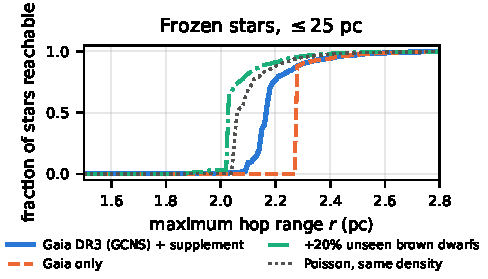
\includegraphics[width=\linewidth]{figures/percolation.pdf}
\caption{Fraction of the \NEval\ stars within \EvalRadius~pc reachable from the
Sun with frozen stars, against the maximum single hop $r$. The transition is
abrupt. With Gaia alone (dashed) the Sun's \PocketGaiaSize-star pocket holds
everything until $r$ reaches \PocketBridge~pc. Unseen brown dwarfs (dash-dot,
+20\%) and a Poisson field of equal density (dotted) shift the threshold
slightly lower.}
\label{fig:percolation}
\end{figure}

\paragraph{The threshold.} Reach jumps from almost nothing to almost everything
over a narrow band of $r$ (Figure~\ref{fig:percolation}). Ten percent of the
stars within \EvalRadius~pc are reachable at $r_{10}=\RTen$~pc, half at
$r_{50}=\RFifty$~pc (bootstrap 95\% CI over Gaia astrometric errors:
\RFiftyLo--\RFiftyHi~pc), and 90\% at $r_{90}=\RNinety$~pc. The median
nearest-neighbour distance is \NNMedian~pc, so a ship must out-range the
typical spacing by a factor of about two. The threshold barely depends on
the evaluation radius: $r_{50}$ lies between \RFiftySweepMin\ and
\RFiftySweepMax~pc for radii of 10--25~pc. This is percolation. A Poisson field
of the same density gives $r_{50}=\RFiftyPoisson$~pc, close to the
infinite-volume continuum value of \RcPoisson~pc \cite{lorenz2001precise}. The
real neighbourhood is \PctAbovePoisson\% harder to cross than random, a mild
cost of its clustering.

\paragraph{The Sun's pocket.} With Gaia alone, the bottleneck for almost every
star is the same hop. The Sun, Proxima, Barnard's star and Ross~154 form an
island whose shortest way out is a \PocketBridge~pc jump from Ross~154. Adding
Luhman~16 and WISE~0855, the two nearest brown dwarfs, both invisible to Gaia,
opens the pocket, and the threshold becomes a property of the whole field. The
lesson is that the \emph{least visible} objects can be the most important
stepping stones. Injecting a random population of unseen brown dwarfs at 20\%
(30\%) of the stellar number, roughly the ratio in the 20-pc census
\cite{kirkpatrick2021field}, lowers $r_{50}$ to \RFiftyBDTwenty\
(\RFiftyBDThirty)~pc, a \PctBDTwenty\% reduction at 20\%.

\paragraph{Route shape.} Just above threshold, at $r_{90}$, the shortest routes
are long detours. The median route flies \StretchMedian$\times$ the
straight-line distance in \HopsMedian\ hops. Section~\ref{sec:engineering}
shows that this regime defeats simple greedy pilots.

\begin{figure}[t]
\centering
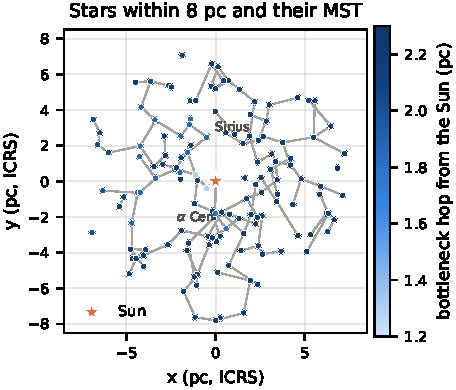
\includegraphics[width=0.92\linewidth]{figures/map.pdf}
\caption{The 3D minimum spanning tree of stars within 8~pc, projected on the
ICRS $x$--$y$ plane, coloured by each star's bottleneck hop from the Sun.
Nearly every star shares the same bottleneck.}
\label{fig:map}
\end{figure}

\section{Moving stars: waiting is a resource}
\label{sec:moving}

\paragraph{A temporal graph with closed-form edges.} Under linear motion the
separation of stars $i$ and $j$ is
$d_{ij}(t)=\lvert p_{ij}+w_{ij}t\rvert$, where $p_{ij}$ is the relative position
at $t=0$ and $w_{ij}$ the relative velocity. Since $d_{ij}^2$ is a convex
quadratic in $t$, a hop of range $r$ is open on \emph{exactly one} interval
$[a_{ij},b_{ij}]$, found in closed form. A ship cruising at $v$ intercepts a
moving target after $\tau$ solving $\lvert p+w\tau\rvert=v\tau$. We open the
edge when $d_{ij}(t)\le r(1-\lvert w\rvert/v)$, which guarantees a flown
distance $\le r$. A colony at $i$, ready at time $t$, leaves at
$\max(t+s,a_{ij})$ if that is $\le b_{ij}$, where $s$ is an optional settling
delay. Leaving later never arrives earlier, so the network is FIFO and
Dijkstra over arrival times is exact \cite{kaufman1993fastest}. Candidate pairs
come from time-sliced KD-tree queries. A unit test checks that no pair whose
separation ever drops below $r$ is missed. A second test checks the arrival
times against a Bellman--Ford fixed point. One run per $r$ yields reach at
every horizon $T$ at once. With $r\le2.25$~pc and $T=1$~Myr the graph has
\TdPairs\ candidate pairs.

\begin{figure*}[t]
\centering
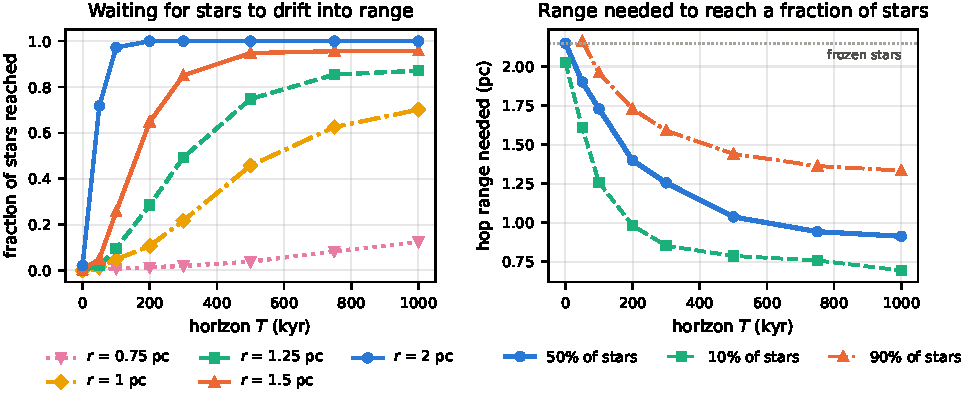
\includegraphics[width=\textwidth]{figures/moving.pdf}
\caption{Moving stars, \TdNEval\ stars within \TdEval~pc, ships at \TdVship~$c$.
\textbf{Left:} fraction reached by horizon $T$ for several hop ranges. Below
the frozen threshold, reach grows steadily as stars drift into range.
\textbf{Right:} range needed to reach 10/50/90\% of stars by time $T$. The band
is the spread over \TdNBoot\ astrometric bootstrap draws. The frozen-star value
is the dotted line.}
\label{fig:moving}
\end{figure*}

\paragraph{Waiting lowers the threshold substantially.} Figure~\ref{fig:moving}
is the central result. If a colony may wait up to 100~kyr, the range needed to
reach half the stars falls from \RFifty\ to \RFiftyTHundred~pc, a
\RedHundred\% reduction (bootstrap range \RedLoHundred--\RedHiHundred\%). The
reduction is \RedTwoHundred\% within 200~kyr, \RedFiveHundred\% within 500~kyr
($r_{50}=\RFiftyTFiveHundred$~pc) and \RedThousand\% within 1~Myr. Our
falsification criterion, a reduction below 5\% at every horizon up to 10~Myr,
is decisively rejected. Stellar motion is not a correction to interstellar
routing. Over $10^5$-year horizons it dominates.

\paragraph{The stars carry the front.} For sub-threshold ranges the expansion
speed is set by stellar motion, not by the ship. With $r=1$~pc, half the stars
within \TdEval~pc are reached at an effective speed of \FrontOne~pc/Myr
(\FrontOneKms~km/s), comparable to the local velocity dispersion. With
$r=1.5$~pc it is \FrontOneHalf~pc/Myr. Naively extrapolated across a
30-kpc Galaxy, these give \GalaxyCrossGyrOne\ and \GalaxyCrossGyrOneHalf~Gyr,
far shorter than the Galaxy's age. This is the Carroll-Nellenback et al.\
\cite{carroll2019fermi} conclusion, obtained here from explicit routes on
measured stars.

\paragraph{What slows it down.} \emph{Settling time} matters most. At
$r=\SweepR$~pc and $T=200$~kyr, \SettleZero\% of stars are reached with
instant relaunch, \SettleTen\% if each colony needs 10~kyr before it can
launch again, and \SettleHundred\% with 100~kyr. \emph{Ship speed} matters less
than one might think: \SpeedMid\% at 0.01~$c$ versus \SpeedFast\% at 0.1~$c$.
Only at 0.001~$c$ (300~km/s, comparable to stellar motions) does reach
collapse, to \SpeedSlow\%.

\paragraph{Boundary check.} Stars that would enter from beyond the catalogue
are missing, so a catalogue-limited run \emph{underestimates} the benefit of
motion. The count of catalogued stars inside \TdEval~pc stays at
\RetFiveHundred\% of its initial value at 500~kyr and drops to \RetThousand\% at
1~Myr. Results beyond 500~kyr are therefore conservative. The full
configuration uses the 100-pc catalogue.

\section{From range to engineering}
\label{sec:engineering}

\paragraph{Propulsion sets speed, lifetime sets range.} A rocket that must
accelerate \emph{and} brake on one tank with mass ratio $R$ and exhaust speed
$v_e$ cruises at $v=c\tanh(v_e\ln R/2c)$ (relativistic rocket equation, half
the rapidity on each burn). Its hop range is $r=v\,\tau_{\max}$, where
$\tau_{\max}$ is how long the ship, or its crew, survives in transit. The
per-hop survival time needed to percolate is therefore $\tau^\ast=r_{50}/v$
(Figure~\ref{fig:propulsion}). At $R=10$, chemical rockets need
\TauChemStatic~yr per hop and high-$I_{\rm sp}$ electric propulsion
\TauElecStatic~yr. A Daedalus-class fusion ship ($v_e=10^4$~km/s, cruising at
\VFusion~km/s, \VFusionPctC\% of $c$) needs \TauFusionStatic~yr, and an
idealised antimatter ship \TauAntiStatic~yr. If colonies can wait up to
\MovingTkyr~kyr for good alignments, every requirement roughly halves (fusion:
\TauFusionMoving~yr). This turns a technology into a reachability statement:
\emph{fusion propulsion and century-scale reliability are enough to percolate
through the solar neighbourhood}.

\begin{figure}[t]
\centering
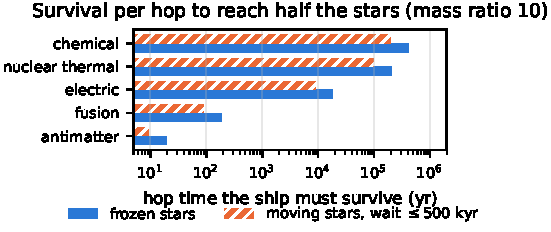
\includegraphics[width=\linewidth]{figures/propulsion.pdf}
\caption{Hop time a ship must survive to reach half the stars within
\EvalRadius~pc, by propulsion technology (mass ratio 10, accelerate and brake
on one tank). Hatched bars: colonies may wait up to \MovingTkyr~kyr for stars
to drift into range.}
\label{fig:propulsion}
\end{figure}

\paragraph{Pilots: greedy fails near threshold, A* is cheap.} On the static
range graph, a greedy geographic pilot (always hop to the in-range neighbour
closest to the target) reaches only \GreedyTwoFive\% of random targets at
$r=2.5$~pc and \GreedyThree\% at 3~pc. It gets stuck in local minima, the
``voids'' known from wireless routing \cite{bose2001routing}. It succeeds
\GreedyFour\% of the time at 4~pc. Near threshold, optimal routes are winding
(median stretch \OptStretchTwoFive\ at 2.5~pc), so a heuristic that never
moves away from the target is wrong by design. A* with the straight-line
heuristic finds the same optimal routes as Dijkstra while expanding a median
of \AstarRatioTwoFive\% of Dijkstra's nodes at 2.5~pc and \AstarRatioFour\% at
4~pc.

\paragraph{Refuelling only where planets are known.} Suppose a ship may stop
anywhere, with hops of at most \FuelHop~pc for crew or hardware reasons, but
can refuel only at the \NHostsFuel\ known exoplanet hosts within
\FuelRadius~pc. The tank range then needed to reach each star is again a
bottleneck, now on a station graph whose edge weights are in-graph shortest
distances. We compute it exactly by multi-source Dijkstra and an MST over
stations. Reaching half the stars needs a \TankFifty~pc tank (90\%:
\TankNinety~pc), \TankRatio$\times$ the \RefuelAnyFifty~pc that suffices when
any star can refuel (Figure~\ref{fig:routing}, left). Planet surveys therefore
shorten the required tank directly: every newly confirmed host is a potential
refuelling station.

\begin{figure*}[t]
\centering
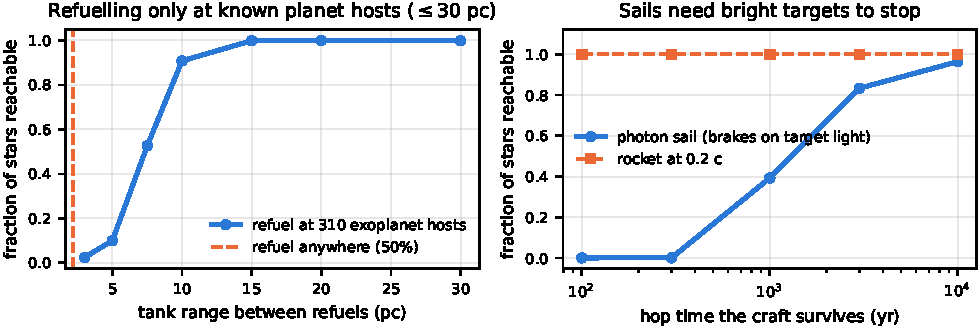
\includegraphics[width=\textwidth]{figures/routing.pdf}
\caption{\textbf{Left:} reach within \EvalRadius~pc against tank range when
refuelling is possible only at known exoplanet hosts (hops $\le$\FuelHop~pc).
The dashed line is $r_{50}$ when any star can refuel. \textbf{Right:} photon
sails launched at \SailVLaunch~$c$ but braking only on the target star's light,
against a rocket flying at the same speed. Reach is plotted against the hop
time the craft survives.}
\label{fig:routing}
\end{figure*}

\paragraph{Sails need bright targets.} A laser-launched sail can leave at
\SailVLaunch~$c$, but to stop it must shed its speed on the target's light.
Scaling the photogravitational braking limit of \cite{heller2017optimized}
(13,800~km/s at $\alpha$~Cen~A) as $L^{0.4}$, the median star within
\EvalRadius~pc can stop a sail arriving at only \SailBrakeMedian~km/s. Only
\SailFracFast\% can stop one faster than 0.01~$c$, because most nearby stars
are M dwarfs. Sail routes therefore hop between bright stars or crawl into dim
ones. With a 1,000-yr hop budget a sail network reaches \SailReachThousand\% of
stars, against 100\% for a rocket at the same cruise speed. At 3,000~yr it
reaches \SailReachThreeThousand\%, and half the stars take \SailTFifty~yr
rather than \RocketTFifty~yr (Figure~\ref{fig:routing}, right).

\paragraph{Exploring everything nearby.} Finally we reproduce the classic
probe-exploration model of Bj{\o}rk \cite{bjork2007exploring}. A fleet splits
the sky into sectors, and each probe visits every star in its sector, here
the \ExNStars\ stars within \ExRadius~pc. Replacing the nearest-neighbour rule
with 2-opt local search shortens total flight by \TwoOptMin--\TwoOptMax\%
across fleet sizes of 1--16, consistent with the $\sim$10\% of
\cite{cotta2009computational} on synthetic stars
(Figure~\ref{fig:exploration}). Against the MST lower bound, nearest-neighbour
tours are \NNGapOne\% too long and 2-opt tours \OptGapOne\%. At 0.1~$c$ a
single probe needs \MakespanOneKyr~kyr to visit them all. A fleet of
\FleetBig\ needs \MakespanEightKyr~kyr. Fleet parallelism, not tour quality,
dominates exploration time.

\begin{figure}[t]
\centering
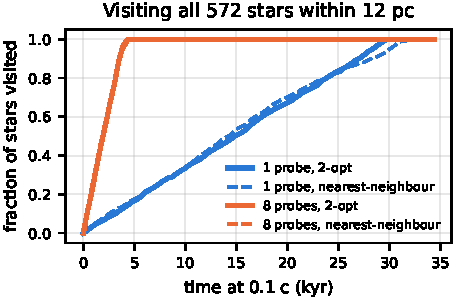
\includegraphics[width=\linewidth]{figures/exploration.pdf}
\caption{Fraction of stars within \ExRadius~pc visited over time by 1 and
\FleetBig\ probes at 0.1~$c$: 2-opt tours (solid) against the nearest-neighbour
rule (dashed).}
\label{fig:exploration}
\end{figure}

\section{Limitations and conclusion}
\label{sec:conclusion}

\paragraph{Limitations.} (i) \emph{Completeness.} Gaia misses most brown dwarfs
and some bright stars. We add the most important ones by hand and bound the
remaining effect by injection, which lowers the threshold by about
\PctBDTwenty\%. The true neighbourhood is therefore somewhat \emph{easier} to
cross than our graph. (ii) \emph{Kinematics.} Stars move on straight lines.
Galactic curvature, binary orbits and close-encounter scattering are ignored.
This is adequate for $\lesssim1$~Myr inside 50~pc but not for Galaxy-scale
extrapolation. (iii) \emph{Missing RVs} are drawn from a conditional velocity
ellipsoid. Their individual values are uncertain, though the statistics are
unbiased. (iv) \emph{Boundaries.} The moving-star results lose inflowing stars
after about 500~kyr and are conservative there. (v) \emph{Engineering} models
are deliberately simple: one range per ship, refuelling as a binary property of
a star, and a sail-braking law scaled from one calibrated case. (vi) We treat
a colony's ability to relaunch as given, with an optional settling delay.
Sociology is out of scope.

\paragraph{Conclusion.} Routed exactly on the measured solar neighbourhood, the
interstellar graph has a sharp percolation threshold near \RFifty~pc per hop,
about twice the typical spacing. That threshold falls by half once ships may
wait $\sim$$10^5$ years for the stars themselves to close the gaps. In this
regime the expansion front moves at stellar speeds. A fusion ship that survives
a couple of centuries per hop crosses the neighbourhood. Sails need luminous
stopping points, and refuelling only at known planet hosts multiplies the
required tank by \TankRatio. The time-dependent formulation is exact, cheap and
scales directly to the 100-pc GCNS and to deeper Gaia releases. Natural next
steps are Galactic-potential orbits, gravitational-assist edges between stars,
and stochastic colony survival.

\paragraph{Reproducibility.} \texttt{make test \&\& make all} in
\texttt{projects/18\_interstellar\_routes} downloads and caches the catalogue,
runs every experiment, and regenerates the figures and every number in this
paper (about 3~minutes on a laptop CPU for the 50-pc configuration).


\FloatBarrier
\bibliographystyle{plain}
\bibliography{references}

\end{document}
